\chapter{Paraphrasing on Deep Syntactic Layer}
\addcontentsline{toc}{chapter}{treex}


In this chapter,\footnote{This chapter is based on the article \citep{barancikova-rosa-2015-targeted}, which is a joint work with Rudolf Rosa. 
Rudolf wrote the two new Treex blocks. My responsibilities included data preparation, paraphrasing and evaluation of experiments.} 
we present a method of targeted paraphrasing of reference sentences on a deep syntactic layer. 
For this purpose, we employ NLP framework Treex and extend it with modules for targeted paraphrasing and word order changes. 
Automatic scores computed using these paraphrased reference sentences show improvement in correlation with human judgment to the original reference sentences.


\section{Introduction}

In this paper, we use deep syntactic layer for targeted paraphrasing of 
reference sentences. For every hypothesis, we create its own reference sentence
that is more similar in wording but keeps the meaning and grammatical
correctness of the original reference sentence. Using these new paraphrased 
references makes the MT evaluation metrics more reliable. In addition, correct 
paraphrases have additional application in many other NLP tasks.

As far as we know, this is the first rule-based model specifically designed for
targeted paraphrased reference sentence generation to improve MT evaluation 
quality.

In the previous chapter, we experimented with targeted paraphrasing using the SMT system Moses,
which we adapted Moses for targeted monolingual phrase-based translation. However, results of this 
method was inconclusive.  

As a next step, we decided to employ rule-based translation system. 
This approach has many advantages, e.g. there is no need for creating a targeting feature and we can change only parts of a sentence and thus create more conservative paraphrases. 
We utilize Treex \cite{treex}, highly modular NLP software system developed for machine translation system TectoMT \cite{tectomt} that translates on a deep syntactic layer. 
Treex is open-source and is available on GitHub,\footurl{https://github.com/ufal/treex} including the two blocks that we contributed. I

\section{Treex}

\begin{figure*}[tb]
\begin{center}
%\scalebox{0.89}{
%\begin{tabular}{l|l}
 \begin{tabular}{l|l}
 Source &  \begin{tabular}{l}
  	\textit{The Internet has caused a boom in these speculations.} \\
	\end{tabular} \\
 \hline
 
 Hypothesis & \begin{tabular}{lllllll}
 			Internet & vyvolal & boom & v  & t\v{e}chto & spekulac\'{i}ch & . \\
 			\textit{Internet} & \textit{caused} & \textit{boom} & \textit{in} & \textit{these} & \textit{speculations} & \textit{.}\\
			\end{tabular} \\
 &  \begin{tabular}{l}
  	\textit{The Internet has caused a boom in these speculations. }\\
	\end{tabular} \\

 \hline
 %\noindent\rule{8cm}{0.4pt}\\
 Reference & \begin{tabular}{llllll}
 			Rozkv\v{e}t & t\v{e}chto & spekulac\'{i} & zp\r{u}sobil & internet & .  \\
 			\textit{Boom} & \textit{these} &  \textit{speculations} & \textit{caused} & \textit{internet} & \textit{.} \\
			\end{tabular} \\
 &  \begin{tabular}{l}
  	\textit{A boom of these speculation was caused by the Internet.} \\
	\end{tabular}  \\ 
%TODO tu ma zas nejaky potize s tim, ze "rozkvet" ma mit spravnou glossu a zpusobit ma byt prelozeno "make.possible", ale mne to prijde jako blbost..
\end{tabular}

\vspace{20pt}

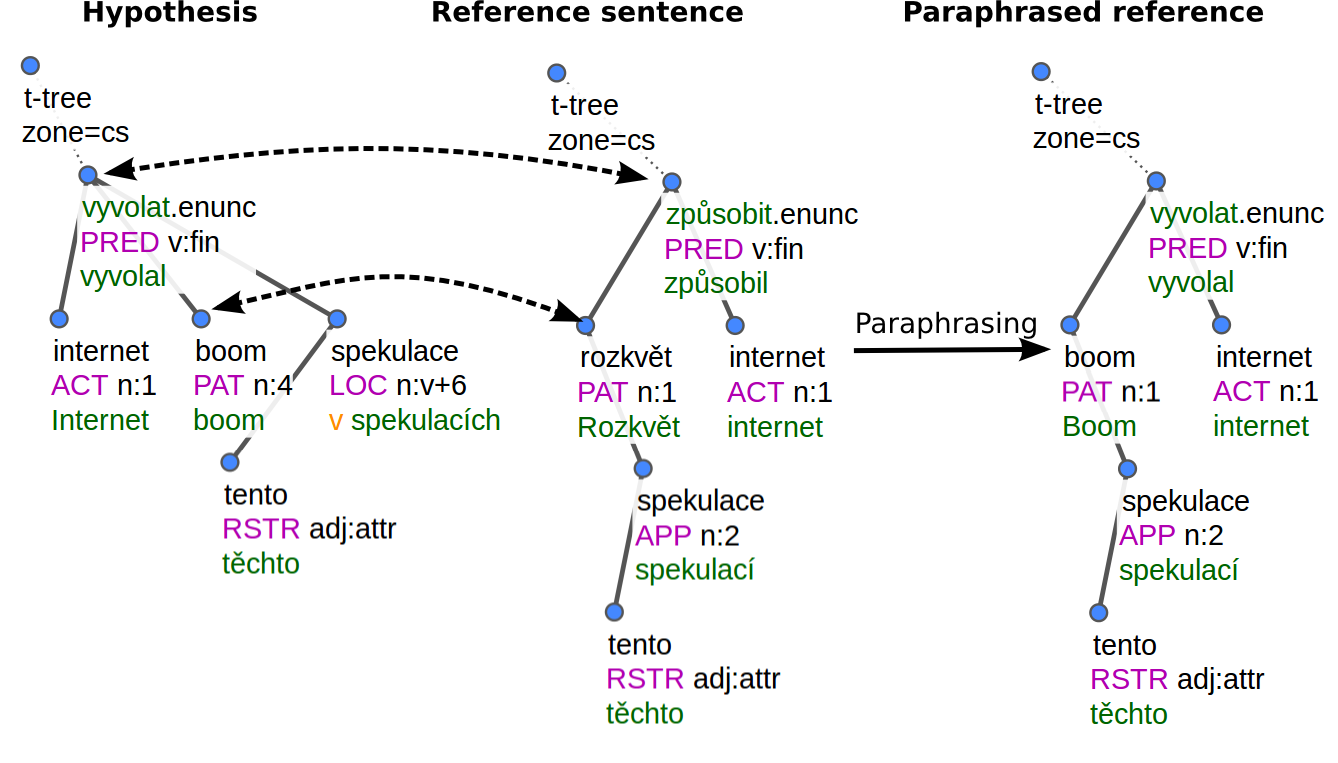
\includegraphics[scale=0.4]{../img/treex_paraphrasing_example.png} 

\caption{Example of the paraphrasing. The~hypothesis is grammatically correct 
and has the same meaning as the reference sentence. We analyse both 
sentences to t-layer, where we create a new reference sentence by substituting
synonyms from hypothesis to the reference. In the next step, we will change also
the word order to better reflect the hypothesis.}
\label{example}
\end{center}
\end{figure*}

Treex implements a stratificational approach to language, adopted from the 
Functional Generative Description theory \cite{FGP} and its later extension by 
the Prague Dependency Treebank \cite{PDT3.0}. It represents sentences at four 
layers:
\begin{itemize}
\item \textbf{w-layer:} word layer; no linguistic annotation
\item \textbf{m-layer:} morphological layer; sequence of tagged and lemmatized 
tokens
\item \textbf{a-layer:} shallow-syntax/analytical layer; sentence is 
represented as a surface syntactic dependency tree
\item \textbf{t-layer:} deep-syntax/tectogrammatical layer; sentence is 
represented as a deep-syntactic dependency tree, where autosemantic words (i.e.
semantically full lexical units) only have their own nodes; t-nodes consist of
a~t-lemma and a~set of~attributes -- a \textit{formeme} (information about the original syntactic form) and a set of \textit{grammatemes} 
(essential morphological features).
\end{itemize} 

We take the analysis and generation pipeline from the TectoTM system. We 
transfer both a hypothesis and its corresponding reference sentence to the 
t-layer, where we integrate a module for t-lemma paraphrasing. After 
paraphrasing, we perform synthesis to a-layer, where we plug in a reordering
module and continue with synthesis to the w-layer. 

\subsection{Analysis from w-layer to t-layer}
The analysis from the w-layer the to a-layer includes tokenization, POS-tagging and 
lemmatization using MorphoDiTa \cite{morphodita}, dependency parsing using the 
MSTParser \citep{McDonald:2005} adapted by \cite{Novak:2007}, trained on PDT.

In the next step, a surface-syntax a-tree is converted into a deep-syntax 
t-tree. Auxiliary 
words are removed, with their function now represented using t-node attributes 
(grammatemes and formemes) of autosemantic words that they belong to (e.g. two
a-nodes of the verb form \textit{spal jsem} (``I slept'') would be collapsed 
into one t-node \textit{spát} (``sleep'') with the tense grammateme set to 
past; \textit{v květnu} (``in May'') would be collapsed into \textit{květen} 
(``May'') with the formeme \textit{v+X} (``in+X'').

%tady zminit proc vlasne chceme parafrazovat pres tektokgramatickou rovinu
% jednak existuji scenare pro cestu tam a dolu a jednak na te rovine jsou slova
% zbavena uz prakticky vsech syntaktickych informaci. 
We choose the t-layer for paraphrasing, because the words from the sentence 
are lemmatized and free of syntactical information. Furthermore, functional 
words, which we do not want to paraphrase and that cause a lot of noise in our 
paraphrase tables, do not appear here.

\begin{figure*}[tb]
\begin{center}
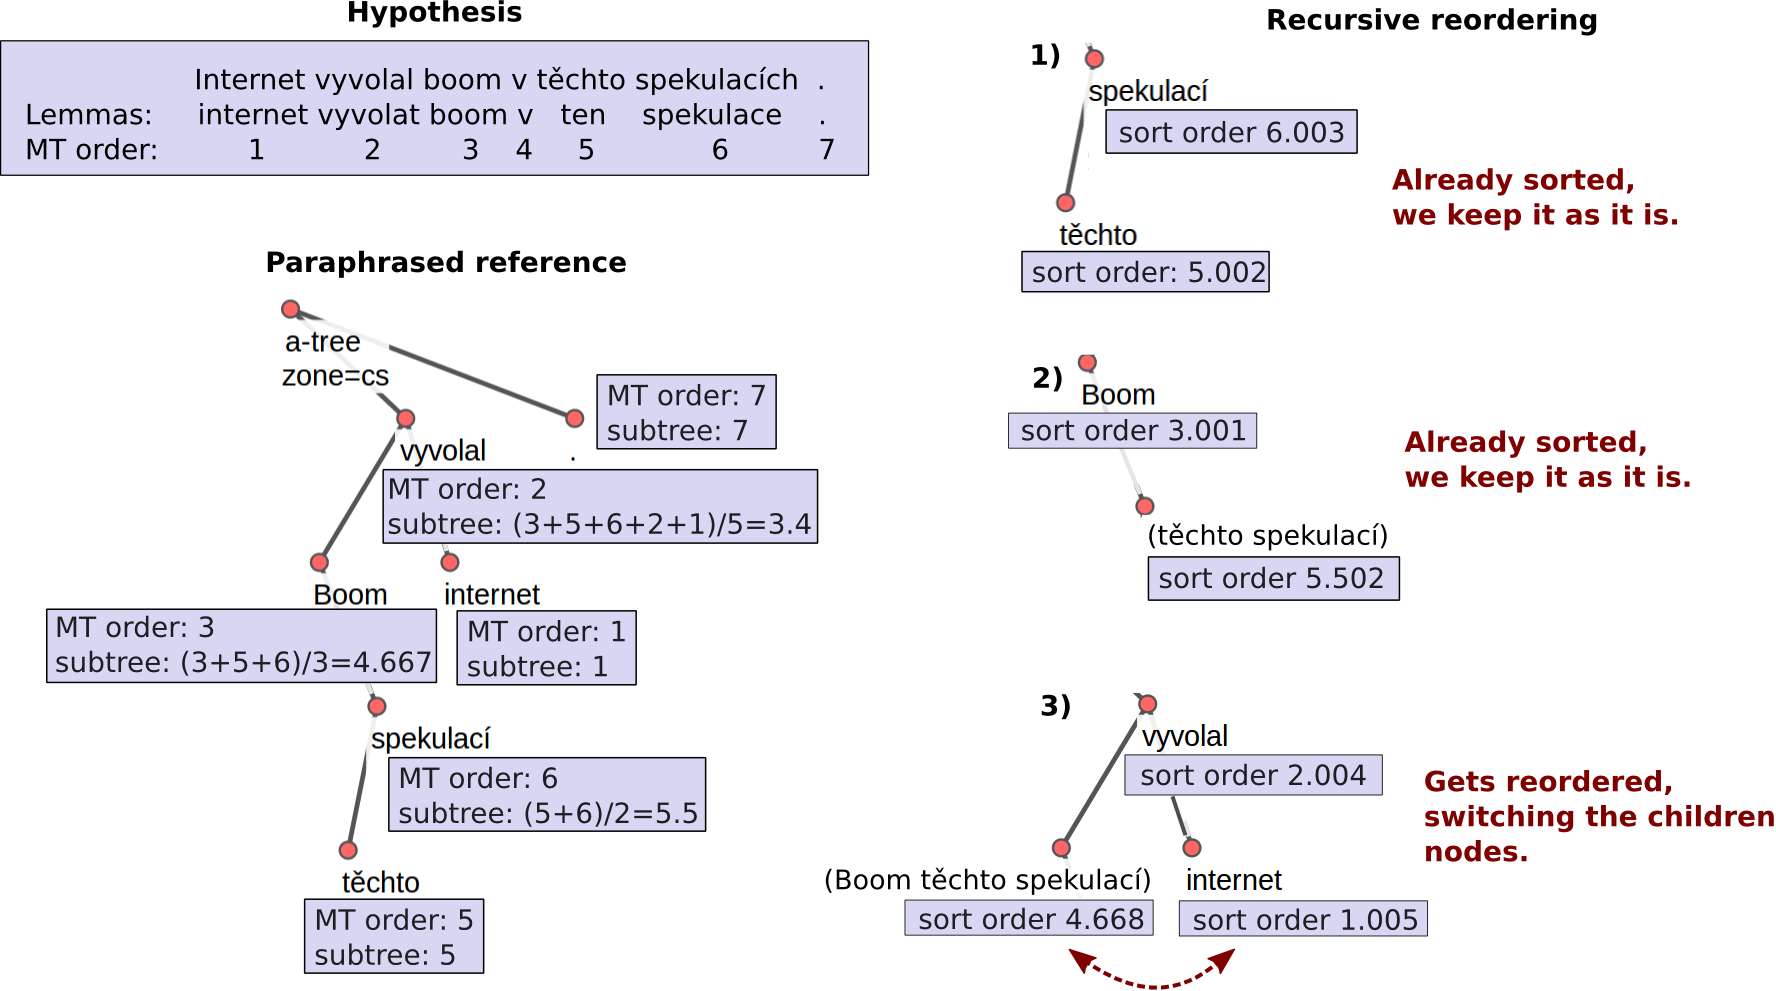
\includegraphics[scale=0.32]{../img/treex_paraphrasing_reordering.png} 
\caption{Continuation of \Fref{example}, reordering of the paraphrased reference
sentence.}
\label{reordering}
\end{center}
\end{figure*}

\subsection{Paraphrasing}
The paraphrasing module T2T::ParaphraseSimple 
is freely available at 
GitHub.\footurl{https://github.com/ufal/treex/blob/master/lib/Treex/Block/T2T/ParaphraseSimple.pm} 

T-lemma of a reference t-node R is changed from A to B if and only if:
\begin{enumerate}
\item there is a hypothesis t-node with lemma B
\item there is no hypothesis t-node with lemma A 
\item there is no reference t-node with lemma B
\item A and B are paraphrases according to our paraphrase tables
\end{enumerate}

The other attributes of the t-node are kept unchanged based on the assumption that
semantic properties are independent of the t-lemma. However, in practice, there 
is at least one case where this is not true: t-nodes corresponding to nouns are 
marked for grammatical %TODO Grammatical gender is not an inflectional category, therefore, it should not correspond to a a grammeme.
gender, which is very often a grammatical property of 
the given lemma with no effect on the meaning (for example, ``a house'' can be 
translated either as a masculine noun \textit{dům} or as feminine noun 
\textit{budova}),
%; we really believe this should be marked on the lemma only, but this is not the case in Treex. 

Therefore, when paraphrasing a t-node that corresponds to a noun, we delete 
the value of the gender grammateme, and let the subsequent synthesis pipeline 
generate the correct value of the morphological gender feature value (which is 
necessary to ensure correct morphological agreement of the noun's dependents, 
such as adjectives and verbs).

\subsection{Synthesis from t-layer to a-layer}
In this phase, a-nodes corresponding to auxiliary words and punctuation are 
generated, morphological feature values on a-nodes are initialized and set to 
enforce morphological agreement among the nodes. Correct inflectional forms based 
on lemma and POS, and morphological features are generated using MorphoDiTa.

\subsection{Tree-based reordering}
The reordering block A2A::ReorderByLemmas is freely available at GitHub.\footurl{https://github.com/ufal/treex/blob/master/lib/Treex/Block/A2A/ReorderByLemmas.pm}

The idea behind the block is to make the word order of the new reference as 
similar to the word order of the translation, but with some tree-based 
constraints to avoid ungrammatical sentences. 

The general approach is to reorder the subtrees rooted at modifier nodes of a 
given head node so that they appear in an order that is on average similar to 
their order in the translation. \Fref{reordering} shows the reordering process 
of the a-tree from \Fref{example}.

%As the ultimate MT quality metric we apply to compare the translation and
%he reference is word based, we align translation and reference words that have
%an identical lemma. Reordering reference words with a lemma that does not
%appear in the translation has little effect on the resulting score given by the
%metric, we thus treat those as unaligned words. %For simplicity, we also treat
%repeated words as unaligned, as it is not straightforward to decide which of 
%the possible alignments to use; however, repeated words are rather rare. 
%TODO future work – align more words.

Our reordering proceeds in several steps. Each a-node has an order, i.e. a 
position in the sentence.  We define the \emph{MT order} of a reference a-node 
as the order of its corresponding hypothesis a-node, i.e. a node with the same 
lemma. 

We set the MT order only if there is exactly one a-node with the given lemma 
in both the hypothesis and the reference. Therefore, the MT order might be 
undefined for some nodes.

In the next step, we compute the \emph{subtree MT order} of each reference 
a-node R as the average 
%TOD0 What is "average order"? mne to teda prijde jasny   
MT order of all a-nodes in the subtree rooted at the 
a-node R (including the MT order of R itself). Only nodes with a defined MT 
order are taken into account, so the subtree MT order can be undefined for 
some nodes. 

Finally, we iterate over all a-nodes recursively starting from the bottom. Head 
a-node $H$ and its dependent a-nodes $D_i$ are reordered if they violate the
\emph{sorting order}. If $D_i$ is a root of a subtree, the whole subtree is 
moved and its internal ordering is kept.

%TODO This description is difficult to follow (at least for me). - Ja ji zkusila napsat co nejsrozumitelnejc, nevim, jak to udelat jeste pochopitelnejsi.
The sorting order of $H$ is defined as its MT order; the sorting order of each 
dependent node $D_i$ is defined as its subtree MT order. If a sorting order of 
a node is undefined, it is set to the sorting order of the node that precedes 
it, thus favouring neighbouring nodes (or subtrees) to be reordered together in 
case there is no evidence that they should be brought apart from each other. 
Additionally, each sorting order is added 1/1000th of the original order of the 
node -- in case of a tie, the original ordering of the nodes is preferred to 
reordering.

We do not handle non-projective edges in any special way, so they always get 
projectivized if they take part in a reordering process, or kept in their 
original order otherwise. However, no new non-projective edges are created
in the process – this is ensured by always moving the subtrees at once.

Please note that each node can take part in at most two reorderings – once
as the $H$ node and once as a $D_i$ node. Moreover, the nodes can be processed 
in any order, as a reordering does not influence any other reordering.

\subsection{Synthesis from a-layer to w-layer}
The word forms are already generated on the a-layer, so there is little to be 
done. Superfluous tokens are deleted (e.g. duplicated commas)%, prepositions are vocalized
the first letter in a sentence is capitalized, and the tokens are 
concatenated (a set of rules is used to decide which tokens should be
space-delimited and which should not).
The example in \Fref{reordering}) results in the following sentence:
\textit{Internet vyvolal boom těchto spekulací} (``The Internet has caused a boom 
of these speculations.''), which has the same meaning as the original reference 
sentence, is grammatically correst and, most importantly, is much more similar in
wording to the hypothesis.

%ref: Rozkvět těchto spekulací způsobil internet.
%mt: Internet vyvolal boom v těchto spekulacích.
%before reordering těchto spekulací vyvolal internet.
%final: Internet vyvolal boom těchto spekulací.

\section{Data}
%We perform our experiments on data sets from the English-to-Czech 
%translation  task of WMT12 \cite{wmt12}, WMT13 \cite{wmt13}. The data 
%sets contain 13/14\footnote{We use only 12 of them because two of them (FDA.2878 
%and online-G) have no human judgments.} files with Czech outputs of MT systems.
%Each data set also contains one file with corresponding reference sentences.

Our database of t-lemma paraphrases was created from two existing sources of 
Czech paraphrases -- the Czech WordNet 1.9 PDT \cite{czech-wordnet} and the 
Meteor Paraphrase Tables \cite{meteor-tables}. Czech WordNet 1.9 PDT is already 
lemmatized, lemmatization of the Meteor Paraphrase tables was performed using 
MorphoDiTa \cite{morphodita}.

We also performed fitering of the lemmatized Meteor Paraphrase tables based on 
coarse POS, as they contained a lot of noise due to being constructed 
automatically.

\section{Results}
\begin{table*}[tb]
\begin{center}


\begin{tabular}{|c|ccc|ccc|}
\hline
\multicolumn{1}{|l|}{} & \multicolumn{3}{c|}{\textbf{WMT12}}   & \multicolumn{3}{c|}{\textbf{WMT13}}  \\ 
\hline
references             & original & paraphrased & reordered & original & paraphrased & reordered \\ 
\hline
BLEU                   & 0.751    & 0.783       & 0.804     & 0.834    & 0.850       & 0.878       \\ 
Meteor                 & 0.833    & 0.864       & 0.868     & 0.817    & 0.871       & 0.870       \\ 
Ex.Meteor              & 0.861    & 0.900  & \textbf{0.903} & 0.848  & \textbf{0.893} & \textbf{0.893} \\ 
\hline
\end{tabular}
\caption{Pearson correlation of a metric and human judgment on original 
references, paraphrased references and paraphrased reordered references. 
Ex.Meteor represents Meteor metric with exact match only (i.e. no paraphrase
support).}
\label{results}
\end{center}
\end{table*}

%The performance of an evaluation metric in MT is usually computed as the
Pearson correlation between the automatic metric and human judgment \cite{bleu}. 
The~correlation estimates the linear dependency between two sets of values. 
It ranges from -1 (perfect negative linear relationship) to 1 (perfect linear 
correlation). 

The official manual evaluation metric of WMT12 and WMT13 provides just a 
relative ranking: a human judge always compares the performance of five systems 
on~a~particular sentence. From these relative rankings, we compute the absolute 
performance of every system using the  “$ > $ others” method \cite{bojar-grains}.
It is computed as $ \frac{wins}{wins+loses} $.

Our method of paraphrasing is independent of an evaluation metric used. We 
employ three different metrics - BLEU score, Meteor metric and Meteor metric 
without the paraphrase support (as it seem redundant to use paraphrases on 
already paraphrased sentences). 
%TODO asi by to chtelo zaradit vic metrik, kdyz se tim tak chlubim
% idealne nejakou tu "hlubokou", napr. semPOS

The results are presented in \Tref{results} as a Pearson correlation of a 
metric with human judgment. Paraphrasing clearly helps to reflect the human 
perception better. Even the Meteor metric that already contains paraphrases
is performing better using paraphrased references created from its own 
paraphrase table. This is again due to the noise in the paraphrase table, which
blurs the difference between the hypotheses of different MT systems.

The reordering clearly helps when we evaluate via the BLEU metric, which 
punishes any word order changes to the reference sentence. Meteor is more
tolerant to word order changes and the reordering has practically no effect 
on his scores.

However, manual examination showed that our constraints are not strong enough 
to prevent creating ungrammatical sentences. The algorithm tends to copy the
word order of the hypothesis, even if it is not correct. Most errors were caused
by changes of a word order of punctuation. 

%16:17 sol2 paraphrasing$cat wmt12.prumer | prumer
%4180.08
%16:17 sol2 paraphrasing$cat wmt13.prumer | prumer
%3548.67
%16:18 sol2 paraphrasing$cat wmt14.prumer | prumer
%3787.2

\section{Future Work}
In our future work, we plan to extend the paraphrasing module for more 
complex paraphrases including %TODO A pretty incongruous collection...
syntactical paraphrases, longer phrases,
diatheses. We will also change only parts of sentences that are 
dependent on paraphrased words, thus keeping the rest of the sentence 
correct and creating more conservative reference sentences.

We also intend to adjust the reordering function by adding rule-based constrains. 
Furthermore, we'd like to learn automatically possible
word order changes from Deprefset \cite{bojar-scratching}, which contains 
an excessive number of manually created reference translations for 50 
Czech sentences.

We performed our experiment on Czech language, but the procedure is generally 
language independent, as long as there is analysis and synthesis support for 
particular language in Treex. Currently there is full support for Czech, 
English, Portuguese and Dutch, but there is ongoing work on many more languages 
within the QTLeap\footurl{http://qtleap.eu/} project.
%and the diathesis grammateme set to passive; 



